% Options for packages loaded elsewhere
\PassOptionsToPackage{unicode}{hyperref}
\PassOptionsToPackage{hyphens}{url}
%
\documentclass[
]{article}
\usepackage{lmodern}
\usepackage{amssymb,amsmath}
\usepackage{ifxetex,ifluatex}
\ifnum 0\ifxetex 1\fi\ifluatex 1\fi=0 % if pdftex
  \usepackage[T1]{fontenc}
  \usepackage[utf8]{inputenc}
  \usepackage{textcomp} % provide euro and other symbols
\else % if luatex or xetex
  \usepackage{unicode-math}
  \defaultfontfeatures{Scale=MatchLowercase}
  \defaultfontfeatures[\rmfamily]{Ligatures=TeX,Scale=1}
\fi
% Use upquote if available, for straight quotes in verbatim environments
\IfFileExists{upquote.sty}{\usepackage{upquote}}{}
\IfFileExists{microtype.sty}{% use microtype if available
  \usepackage[]{microtype}
  \UseMicrotypeSet[protrusion]{basicmath} % disable protrusion for tt fonts
}{}
\makeatletter
\@ifundefined{KOMAClassName}{% if non-KOMA class
  \IfFileExists{parskip.sty}{%
    \usepackage{parskip}
  }{% else
    \setlength{\parindent}{0pt}
    \setlength{\parskip}{6pt plus 2pt minus 1pt}}
}{% if KOMA class
  \KOMAoptions{parskip=half}}
\makeatother
\usepackage{xcolor}
\IfFileExists{xurl.sty}{\usepackage{xurl}}{} % add URL line breaks if available
\IfFileExists{bookmark.sty}{\usepackage{bookmark}}{\usepackage{hyperref}}
\hypersetup{
  pdftitle={FinalProject},
  pdfauthor={Megan Willis-Jackson},
  hidelinks,
  pdfcreator={LaTeX via pandoc}}
\urlstyle{same} % disable monospaced font for URLs
\usepackage[margin=1in]{geometry}
\usepackage{graphicx,grffile}
\makeatletter
\def\maxwidth{\ifdim\Gin@nat@width>\linewidth\linewidth\else\Gin@nat@width\fi}
\def\maxheight{\ifdim\Gin@nat@height>\textheight\textheight\else\Gin@nat@height\fi}
\makeatother
% Scale images if necessary, so that they will not overflow the page
% margins by default, and it is still possible to overwrite the defaults
% using explicit options in \includegraphics[width, height, ...]{}
\setkeys{Gin}{width=\maxwidth,height=\maxheight,keepaspectratio}
% Set default figure placement to htbp
\makeatletter
\def\fps@figure{htbp}
\makeatother
\setlength{\emergencystretch}{3em} % prevent overfull lines
\providecommand{\tightlist}{%
  \setlength{\itemsep}{0pt}\setlength{\parskip}{0pt}}
\setcounter{secnumdepth}{-\maxdimen} % remove section numbering

\title{FinalProject}
\author{Megan Willis-Jackson}
\date{10/13/2020}

\begin{document}
\maketitle

\hypertarget{cost-of-housing-in-massachusetts}{%
\section{Cost of Housing in
Massachusetts}\label{cost-of-housing-in-massachusetts}}

\hypertarget{introduction}{%
\subsection{Introduction}\label{introduction}}

The research question I will be exploring is how housing prices are
affected by the following variables:

\begin{enumerate}
\def\labelenumi{\arabic{enumi}.}
\tightlist
\item
  Mode of transportation (cateogrical)
\item
  Educational attainment (categorical)
\item
  Commute time to work (continuous)
\item
  Monthly household income (continuous)
\end{enumerate}

This research question is important to understand how various factors
impact how much a person will spend on housing. It will be interesting
to theorize about tradeoffs that may or may not be supported by the
data, for example if a person makes a choice to take a longer commute in
order to pay less in rent, or if they will pay more to be within walking
distance of their job as opposed to needing to drive.

\hypertarget{hypothesis}{%
\subsubsection{Hypothesis}\label{hypothesis}}

The hypothesis that I will test is that the shorter an MA resident's
commute, the more they pay in rent. I will also test the hypothesis that
people who commute via driving tend to pay less in rent than those who
use other modes. I will test whether there is a positive correlation
between monthly income and housing costs, as well as whether any
relationship exists between educational attainment and housing costs.

\hypertarget{data}{%
\subsection{Data}\label{data}}

My dataset is drawn from the 2018 ACS and includes all MA residents who
a) make more than \$0 in monthly income, b) pay more than \$0 in monthly
housing costs, and c) commute longer than 0 minutes to work.

\hypertarget{data-transformations}{%
\subsubsection{Data Transformations}\label{data-transformations}}

My analysis includes the five variables listed above. The housing price
variable is a combination of three variables within ACS: rent, first
mortgage, and second mortgage. Each individual in the dataset pays
either a rent or a mortgage, and those who pay a first mortgage may also
pay a second mortgage. Therefore, this variable may be correlated with
real estate value, but is a bit more nuanced because a person living in
a home worth a certain amount of money may pay less per month than
another person living in a home worth less money because the latter may
pay a mortgage and a second mortgage, for example.

Education attainment is provided in the ACS as over twenty levels. I
have further binned these categories into ``High School or Lower,'' and
``Post-High School,'' as I anticipated this would be the most meaningful
divide in terms of differences between the two populations.

\hypertarget{variable-summary-statistics}{%
\subsubsection{Variable Summary
Statistics}\label{variable-summary-statistics}}

Summary statistics for the variables are included below to provide a
clearer picture of the sample being examined.

\includegraphics{FinalProject_files/figure-latex/histograms - travel time-1.pdf}

\includegraphics{FinalProject_files/figure-latex/histogram, household income-1.pdf}

\includegraphics{FinalProject_files/figure-latex/household cost-1.pdf}

\begin{verbatim}
##  [1] "Car, truck, or van"                                     
##  [2] "Subway or elevated"                                     
##  [3] "Walked"                                                 
##  [4] "Railroad"                                               
##  [5] "Bus or trolley bus"                                     
##  [6] "Streetcar or trolley car (carro publico in Puerto Rico)"
##  [7] "Bicycle"                                                
##  [8] "Other method"                                           
##  [9] "Taxicab"                                                
## [10] "Ferryboat"                                              
## [11] "Motorcycle"
\end{verbatim}

\begin{verbatim}
## [1] "Of the 11 various modes of transport that MA residents use for their commute, the one with the highest percentage of MA residents in our sample is Car, Truck, or Van, which about 82 percent of the sample population uses. We can say with 95% confidence that the true percent of MA residents who use a car, truck, or van for their commute is between 81.4 and 82.3 percent."
\end{verbatim}

\hypertarget{highest-level-of-education}{%
\subsection{Highest Level of
Education}\label{highest-level-of-education}}

\begin{verbatim}
## [1] "Of the 24 various levels of education, the one with the highest percentage of MA residents in our sample is Bachelor's Degree, which about 29 percent of the sample population holds. We can say with 95% confidence that the true percent of MA residents who hold a Bachelor's Degree as their highest level of education is between 28.1 and 29.2 percent."
\end{verbatim}

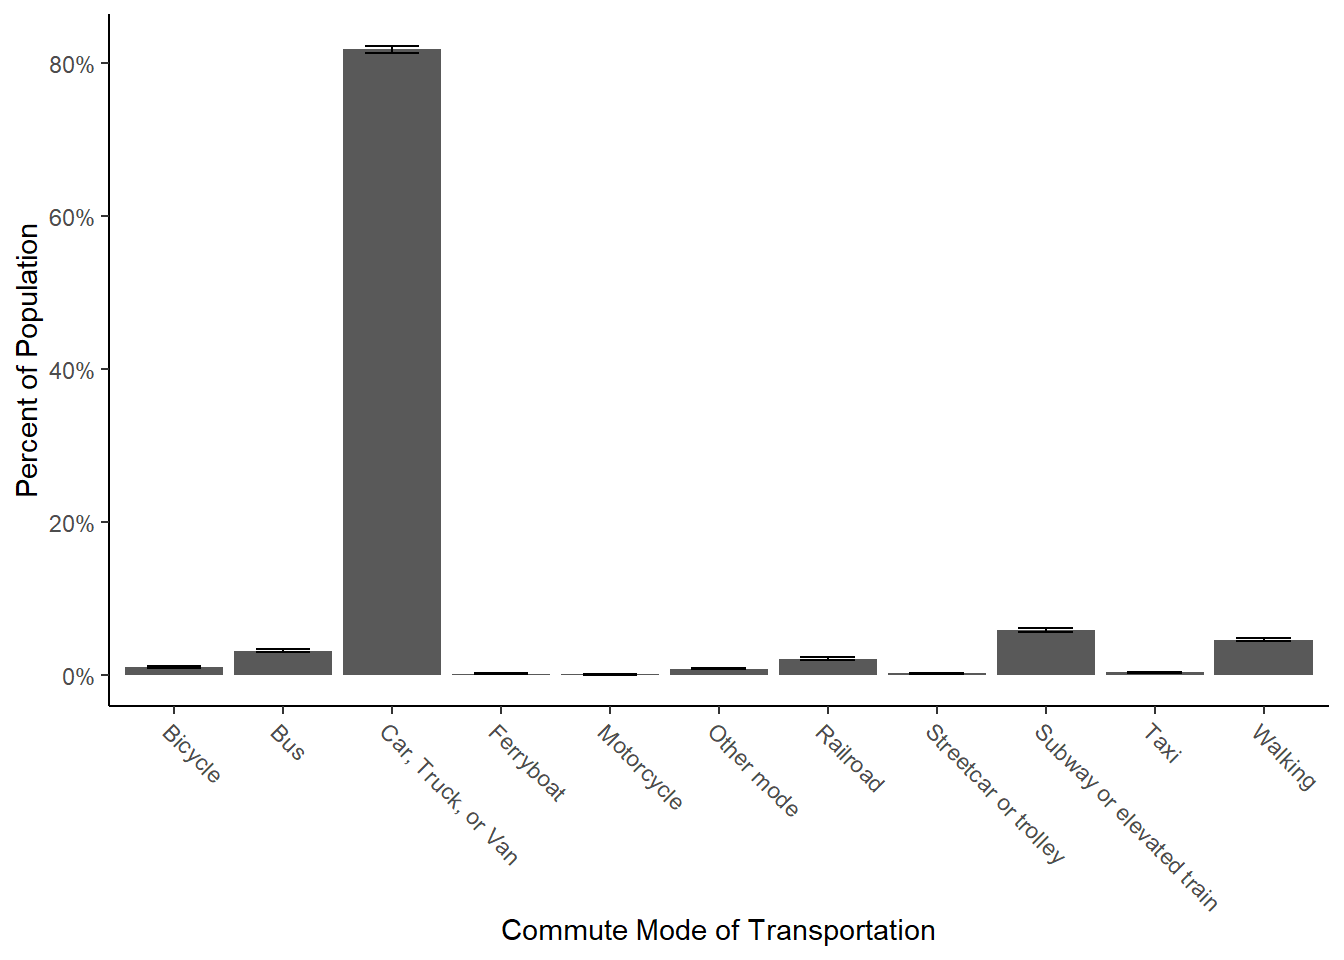
\includegraphics{FinalProject_files/figure-latex/visualize categorical variables - transportation-1.pdf}

\includegraphics{FinalProject_files/figure-latex/visualize categorical variables - education-1.pdf}

\hypertarget{methods}{%
\subsection{Methods}\label{methods}}

I used a variety of statistical tests to explore my hypothesis. These
tests included two sample t-tests, correlations, chi-square tests, and
linear regressions. For each test, a p-value of less than 0.05 indicated
a relationship at the 95\% confidence level, which I took as strong
enough evidence that I should not reject my alternative hypothesis. The
linear regression model analyzes the data hollistically as opposed to
relationships between just two variables, so this is likely the most
useful model to predict relationships between my selected variables. As
each of the t-tests and correlations I examined yielded a p-value of
less than 0.05, I feel it is appropriate to include each of them in the
linear regression. Below, I present some of the t-tests and the linear
regression I performed to paint a picture of housing prices in MA.

\hypertarget{relationship-between-monthly-housing-cost-and-level-of-education}{%
\subsubsection{Relationship between Monthly Housing Cost and Level of
Education}\label{relationship-between-monthly-housing-cost-and-level-of-education}}

We can be 95\% confident that MA residents with some form of higher
education pay, on average, between \$503 to \$549 more per month for
housing than MA residents without any form of higher education.

\begin{verbatim}
## 
##  Welch Two Sample t-test
## 
## data:  travel_time by education_binary == "Post HS"
## t = -16.409, df = 15808, p-value < 2.2e-16
## alternative hypothesis: true difference in means is not equal to 0
## 95 percent confidence interval:
##  -5.617298 -4.418489
## sample estimates:
## mean in group FALSE  mean in group TRUE 
##            27.70165            32.71955
\end{verbatim}

\begin{center}\includegraphics{FinalProject_files/figure-latex/commute and education-1} \end{center}

We can be 95\% confident that MA residents with some form of higher
education pay, on average, between \$503 to \$549 more per month for
housing than MA residents without any form of higher education.

\begin{verbatim}
## 
##  Welch Two Sample t-test
## 
## data:  monthly_housing_total by education_binary == "Post HS"
## t = -44.375, df = 20517, p-value < 2.2e-16
## alternative hypothesis: true difference in means is not equal to 0
## 95 percent confidence interval:
##  -549.2346 -502.7666
## sample estimates:
## mean in group FALSE  mean in group TRUE 
##            1432.824            1958.824
\end{verbatim}

\begin{center}\includegraphics{FinalProject_files/figure-latex/housing and education-1} \end{center}

\hypertarget{linear-regression}{%
\subsubsection{Linear Regression}\label{linear-regression}}

Below I present the results of my linear regression. This model seeks to
predict the relationship between monthly housing costs and mode of
commute, level of educational attainment, household income, and travel
time. It additionally examines how the interaction between mode of
commute and travel time may affect housing costs, because I think there
may be an interaction between people's travel time and mode of commute;
for example, it intuitively would be much rarer for a person to choose
to walk to work for 1.5 hours if they had an option of driving for 30
minutes. In this regression, mode of commute is binned into four
categories which includes driving as the base case (car, truck, or van;
taxi; or motorcycle); public transit; walking/biking; and other.

To me, this interaction is really quite interesting. While the
regression results of the transportation mode variable without the
interaction indicate at the 95\% confidence level that people using each
of the modes of transportation (walk/bike, public transit, and other)
pay a couple of hundred dollars more in housing costs per month than a
person who drives (all else being equal), as travel time increases, the
average person pays more if they drive a car whereas their monthly
housing costs decrease if they use any of the other mode categories.

This model has an R-squared value of 0.249, meaning it explains almost
25\% of the variances in monthly housing costs for MA residents.

The model also suggests that:

\begin{enumerate}
\def\labelenumi{\arabic{enumi}.}
\tightlist
\item
  A person with an education above a high school degree pays about \$276
  more in housing costs than a person with no education above a high
  school degree, all else being equal.
\item
  For every minute increase in time spent commuting, an MA resident pays
  about \$2.26 more in housing costs, all else being equal.
\item
  The longer a person commutes using a mode other than driving, the less
  they tend to pay in housing costs, all else equal.
\item
  And, contrary to what number 3 may suggest, using a mode other than
  driving to commute predicts that a person will pay more in housing
  costs, all else being equal.
\end{enumerate}

\begin{verbatim}
## 
## Call:
## lm(formula = monthly_housing_total ~ transpo_categories + education_binary + 
##     household_income + travel_time + transpo_categories:travel_time, 
##     data = people_mutated)
## 
## Residuals:
##     Min      1Q  Median      3Q     Max 
## -5901.4  -525.8   -90.1   412.0  6281.3 
## 
## Coefficients:
##                                                  Estimate   Std. Error t value
## (Intercept)                                  940.69819045  13.32897896  70.575
## transpo_categoriesother                      249.51034917  82.34040670   3.030
## transpo_categoriespublic transit             390.94399081  36.29843299  10.770
## transpo_categorieswalk/bike                  368.58959790  37.27263700   9.889
## education_binaryPost HS                      276.80892452  12.33261024  22.445
## household_income                               0.00376374   0.00004611  81.633
## travel_time                                    2.25725015   0.27232764   8.289
## transpo_categoriesother:travel_time           -4.46446500   1.53165145  -2.915
## transpo_categoriespublic transit:travel_time  -3.96963477   0.68726488  -5.776
## transpo_categorieswalk/bike:travel_time       -4.52630546   1.57405636  -2.876
##                                                          Pr(>|t|)    
## (Intercept)                                  < 0.0000000000000002 ***
## transpo_categoriesother                                   0.00245 ** 
## transpo_categoriespublic transit             < 0.0000000000000002 ***
## transpo_categorieswalk/bike                  < 0.0000000000000002 ***
## education_binaryPost HS                      < 0.0000000000000002 ***
## household_income                             < 0.0000000000000002 ***
## travel_time                                  < 0.0000000000000002 ***
## transpo_categoriesother:travel_time                       0.00356 ** 
## transpo_categoriespublic transit:travel_time        0.00000000773 ***
## transpo_categorieswalk/bike:travel_time                   0.00404 ** 
## ---
## Signif. codes:  0 '***' 0.001 '**' 0.01 '*' 0.05 '.' 0.1 ' ' 1
## 
## Residual standard error: 900.2 on 27217 degrees of freedom
## Multiple R-squared:  0.2492, Adjusted R-squared:  0.249 
## F-statistic:  1004 on 9 and 27217 DF,  p-value: < 0.00000000000000022
\end{verbatim}

\begin{center}\includegraphics{FinalProject_files/figure-latex/linear regression-1} \end{center}

\hypertarget{discussion}{%
\subsection{Discussion}\label{discussion}}

To restate my initial hypothesis, I was testing whether the shorter an
MA resident's commute, the more they pay in rent; people who commute via
driving tend to pay less in rent than those who use other modes; and
whether there is a positive correlation between monthly income and
housing costs, as well as whether any relationship exists between
educational attainment and housing costs.

The results of my linear regression suggest that there is a positive
correlation between travel time and housing costs. For each additional
minute spent commuting, an MA resident will pay on average an additional
\$2.26 in housing costs, holding all else equal, which does not support
my hypothesis. That result is significant at the 95\% confidence
interval. The results of the linear regression do support the hypothesis
that MA residents who drive tend to pay less in rent than those who use
other modes (all else being equal), which we can say with 95\%
confidence. Of note, however, is that when examining the interaction
between travel time and travel mode, each minute longer spent commuting
tends to decrease the amount spent on housing for all modes except for
driving, which increases. This suggests that, in the context of
Massachusetts, residents living farther from their jobs who drive choose
to pay more to live farther away; perhaps access to the larger, more
expansive real estate farther from the city is the cause.

If I were to investigate this further, I would like to add in a variable
on urban, suburban, and rural housing to control for that (assuming real
estate tends to be more expensive in the city), as well as distance from
one's job, not just time spent commuting. The most glaring weakness in
this analysis is the low number of variables it includes. There are so
many variables which likely have an effect on housing costs; to figure
out how to best improve my analysis, I would conduct background research
on what these variables are.

\hypertarget{conclusion}{%
\subsection{Conclusion}\label{conclusion}}

This analysis is important because, as urban planners intending to
improve the lives of people in a variety of communities, it is
beneficial to know how the factors examined here interact with each
other given that they have a relatively big impact on quality of life.
Is there an ideal trade-off between time spent commuting and housing
costs? Would a person appreciate less time spent in traffic if they were
able to walk? Time and money are arguably two of the biggest things
weighing on people's minds as they make decisions in their lives, so
having an indication of what the trade-offs between them are serve to
help urban planners make decisions within their communities.

\end{document}
